\subsection{Discretization of the Controller}\label{ssec:discnController}
The discretization process of a controller consists in using the map from the continuous domain to the discrete domain (z-domain), with respect to the sampling time, \si{T}, of the feedback control system:
%
\begin{flalign} 
  &\si{s = j \omega \to z = e^{s T}}\label{exp:cont2Disc}&
\end{flalign}
%
Since, by definition, the discrete domain cannot represent the complete behavior of a system through time, approximations are used to estimate this behavior.

One of the most commonly used aproximations is the bilinear transform (or Tustin's method) which is based on the trapezoidal integration principle. A reason to use this method instead of others is that it maps the entire LHP (stable area in the continuous domain) into the unit circle (stable area in the discrete domain)\cite{GFranklin}.\\
The bilinear approximation of \si{z} is defined as:
%
\begin{flalign} 
  &\si{z \approx \frac{1 + s \frac{T}{2}}{1 - s\frac{T}{2}}}\label{exp:bilinearTransform}&
\end{flalign}
%
The inverse transformation of \expr{exp:bilinearTransform} is given by:
%
\begin{flalign} 
  &\si{s \approx \frac{T}{2} \cdot \frac{1 - z^{-1}}{1 + z^{-1}}}\label{exp:inverseBilinearTransform}&
\end{flalign}
%
In general, the \expr{exp:inverseBilinearTransform} is used to replace \si{s} in the continuous-time transfer function of the designed controller. However, due to the non-linear mapping induced by the discretization, a pre-warp of the frequencies can be used before. This avoids effects of phase lag near the cross-over frequency and thus, also avoids unwanted reduction of gain and phase margins, see \cite{GGu,AVOppenheim}. 

Moreover, Matlab has an available function, \lstinline{c2d()}, designed to convert a continuous system's transfer function into the discrete domain by specifying the sampling time (here, \si{T = 0.01s}\fxnote{A justification fo this sampling time should be added at some point.}) and the desired method. The \lstinline{'prewarp'} option that is used, needs a supplementary argument corresponding to the critical fequency, chosen here to be \si{33,5\ rad \cdot s^{-1}}, see \cite{Matlabc2d}.

Figref{fig:bodePrewarpVsNoPrewarpVsContinuous} shows a Bode plot comparing the original continuous controller's frequency and phase responses with the discretized controller's with both normal Tustin's method and pre-warping.
\fxnote{Insert correct figure}
% 
\begin{minipage}{\linewidth}
  \begin{minipage}{0.45\linewidth}
    \begin{figure}[H]
      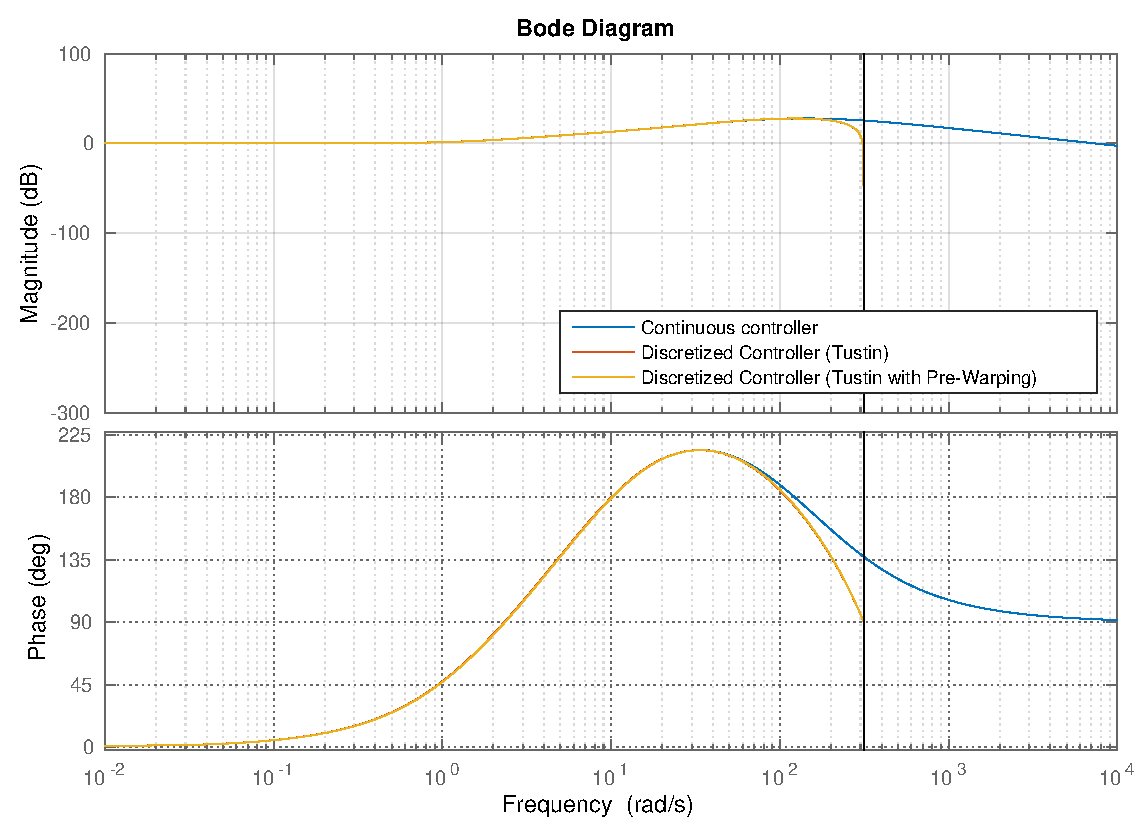
\includegraphics[scale=.50]{figures/prewarpVsNoPrewarpVsContinuousBode.pdf}
      \centering
      \captionsetup{justification=centering}
      \captionof{figure}{Bode plot of the continuous controller (in blue), discretized controller (in red) and pre-warped discretized controller (in orange)}.
      \label{fig:bodePrewarpVsNoPrewarpVsContinuous}
    \end{figure}\vspace{-5mm}
  \end{minipage}
  \hspace{0.03\linewidth}
  \begin{minipage}{0.45\linewidth}
    \begin{figure}[H]
      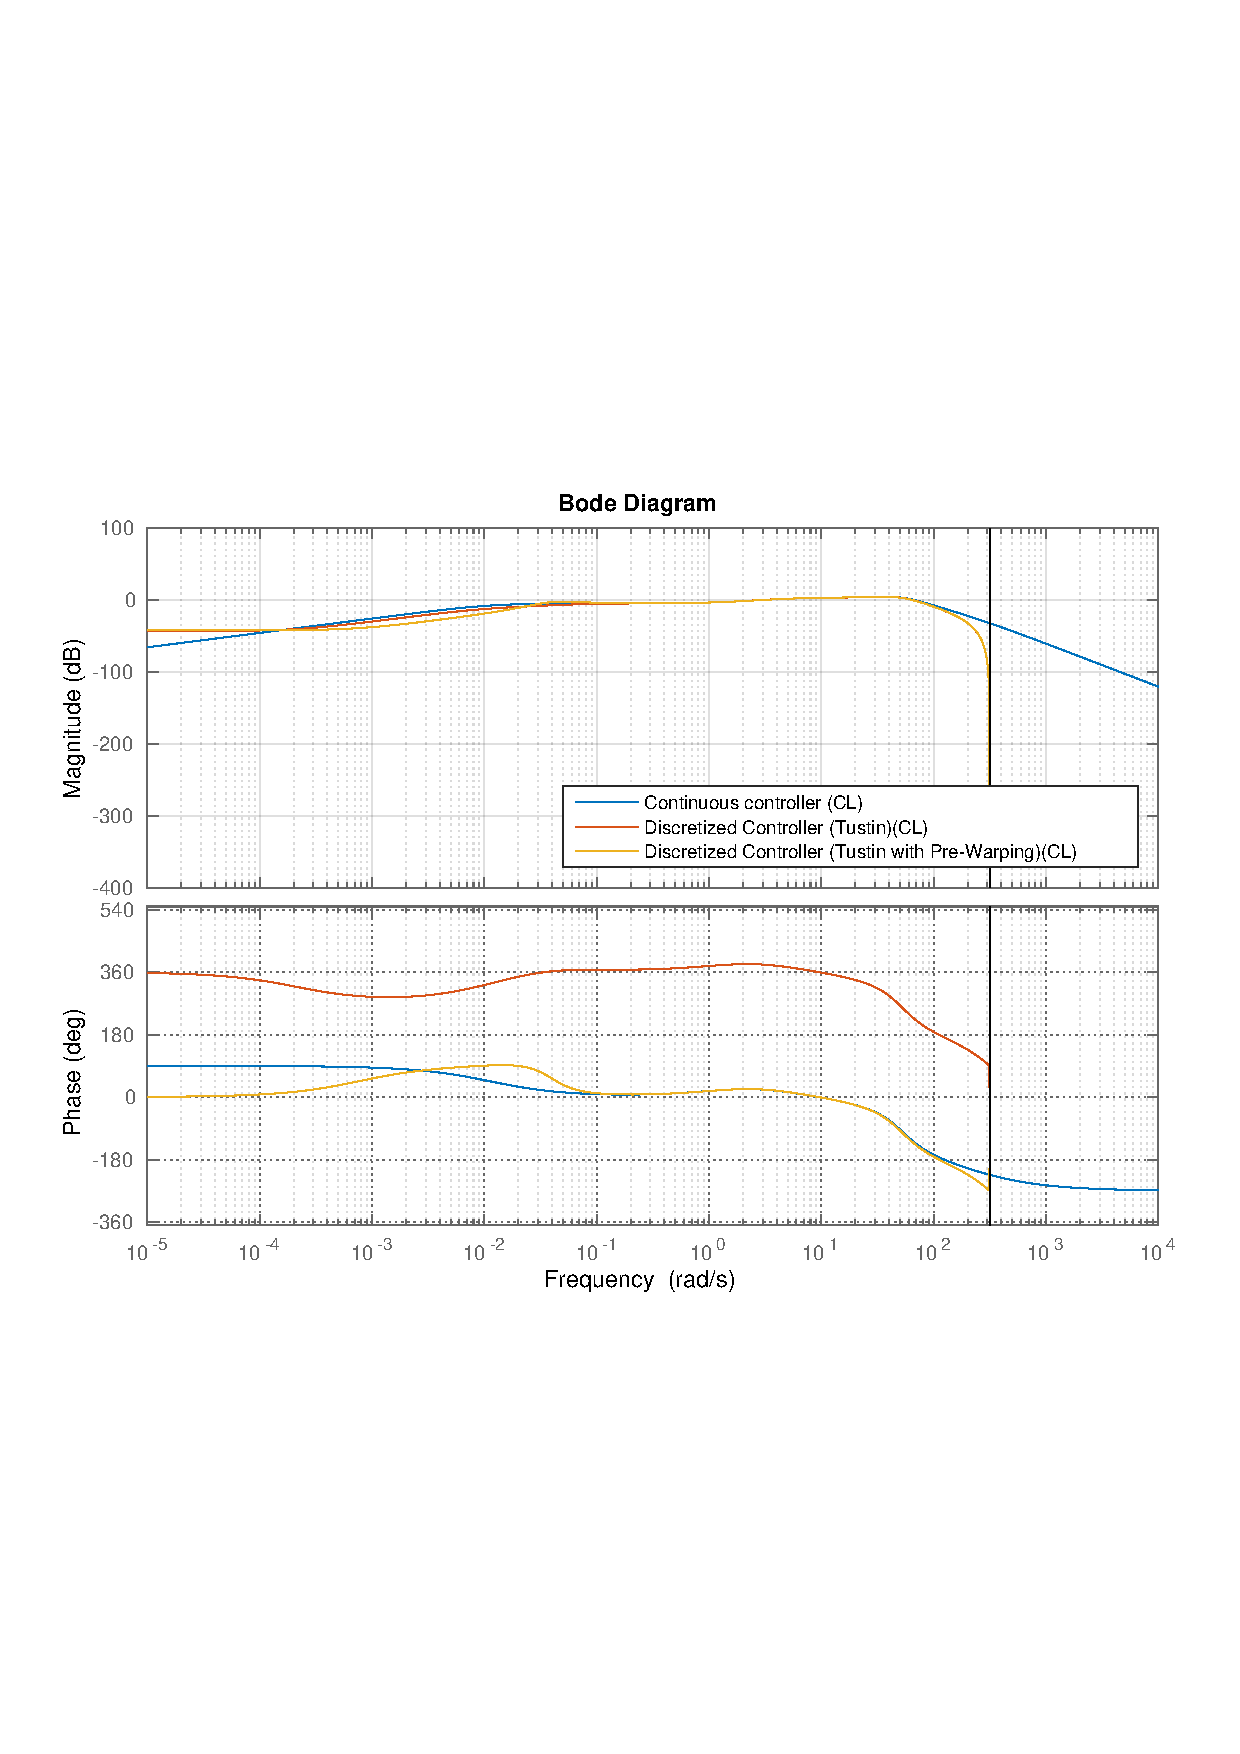
\includegraphics[scale=.50]{figures/prewarpVsNoPrewarpVsContinuousBodeClosedLoop.pdf}
      \centering
      \captionsetup{justification=centering}
      \captionof{figure}{Bode plot of the closed loop system with the continuous controller (in blue), discretized controller (in red) and pre-warped discretized controller (in orange)}.
      \label{fig:bodePrewarpVsNoPrewarpVsContinuousClosedLoop}
    \end{figure}\vspace{-5mm}
  \end{minipage}
\end{minipage}

From figref{fig:bodePrewarpVsNoPrewarpVsContinuous}, it is possible to see...

Thus, the pre-warped discretized controller is chosen for the actual implementation on the Cubli, in the code base, see \secref{sec:codeBase}, and its discrete transfer function is:
\begin{flalign}
  \eq{J_m \cdot \dot{\omega}_m(t)} {\tau_m(t) - B_m \cdot \omega_m(t) - r_m \cdot f_c(t)}%\unit{N \cdot m} 
  \label{eq:discControllerTf}
\end{flalign}
To implement a discrete controller in a code environment, the preferred form is the difference equation:
\begin{flalign}
  \eq{\tau_{m,w}[n]}{}\unit{N \cdot m} 
  \label{eq:discControllerDiffEq}
\end{flalign}
%
\hspace{6mm} Where:\\
\begin{tabular}{ p{1cm} l l l}
& \si{\tau_{m,w}}         & is the wanted motor torque                            &\unitWh{kg \cdot m^2} \\
& \si{e_{\theta}}         & is the error between wanted and measured frame angle  &\unitWh{rad}\\
& \si{n}                &   &\unitWh{\cdot}\\
\end{tabular}

In this subsection, the designed controller has been discretized. The next subsection goes into further analysis of the new feedback control system before the actual implementation on the real system.